\section{Introduction}

%\begin{table}
%   \centering
%   \small
%   \begin{tabular}{|c!{\vrule width .8pt}c!{\vrule width .8pt}c|}
%      \hline
%      \textbf{Approach} & \textbf{Time Complexity} & \textbf{Optimality \wrt QOP} \\
%      \noalign{\hrule height .8pt}
%      Split & \cellcolor{green!30}$\Bigo(3^n)$ & \cellcolor{red!30}greedy, locally optimal \\
%      \hline
%      Holistic & \cellcolor{red!30}$\Bigo(n!)$ & \cellcolor{green!30}globally optimal \\
%      \hline
%   \end{tabular}
%   %\vspace*{.2cm}
%   \caption{Comparison of both optimization approaches.}
%   \label{tbl:pro-cons}
%\end{table}

\begin{figure}[!th]
    \centering
    \begin{subfigure}[b]{\columnwidth}
       \centering
       \includegraphics{/mutable/paper/fig/solution_space.pdf}
       \vspace*{\captiongap}
       \vspace*{\captiongap}
       \caption{Solution space \wrt QOP.}% of the different approaches to solve QOP.  \holistic always finds the globally optimal QEP while requiring more optimization time than \split.  The hybrid approach \topk spans a continuum between both.}
       \label{fig:overview-solution_space}
    \end{subfigure}
    \begin{subfigure}[b]{\columnwidth}
       \vspace{5pt}
       \hspace*{-8pt}
       \centering
       \footnotesize
       \definecolor{c_turquiose}{rgb}{0.28, 0.82, 0.8}
       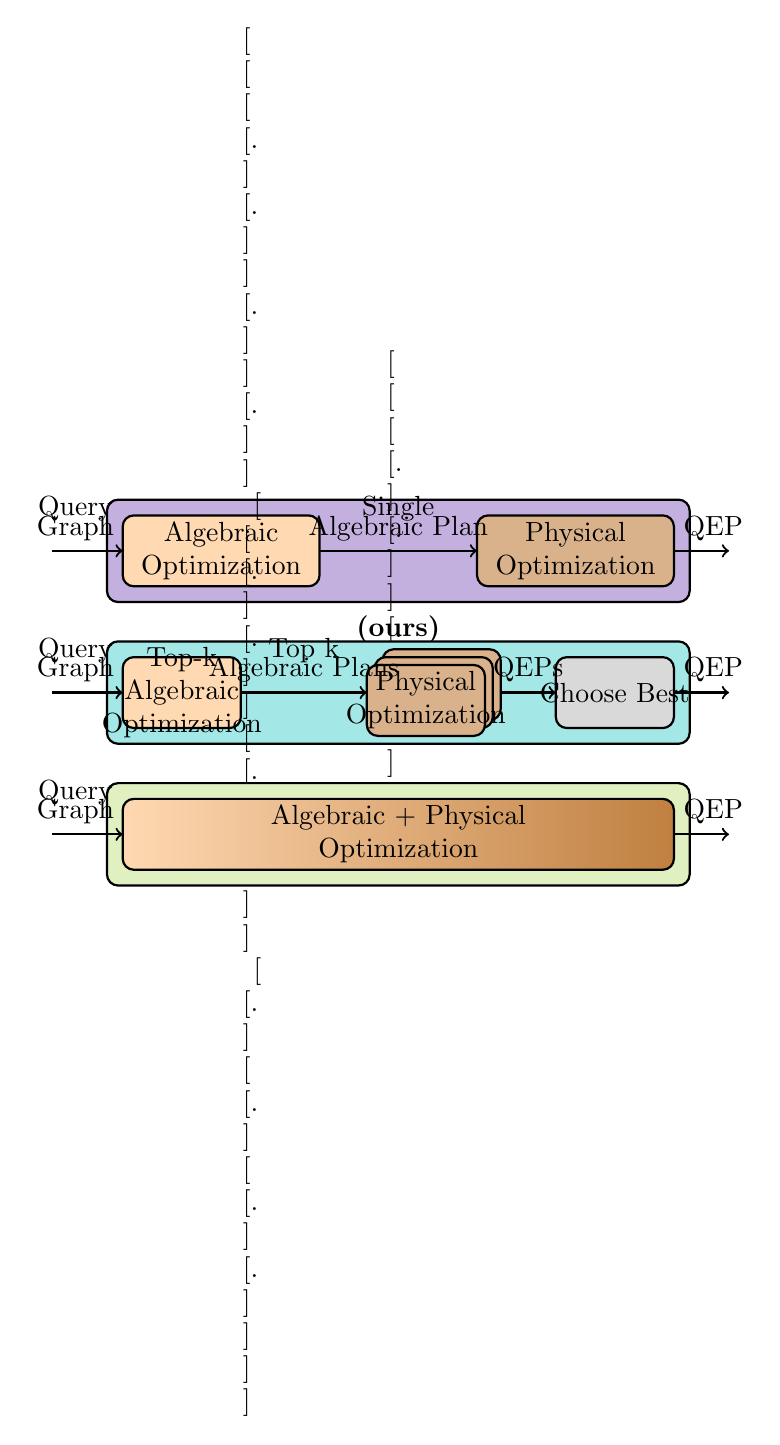
\begin{tikzpicture}[
          box/.style={draw=black, thick, align=center, rounded corners, minimum height=2em},
          arrow/.style={->, draw=black, thick}
       ]
          \node[font=\bfseries] at (3.7,5.05) {\split};
          \draw[box, fill=RoyalPurple!30] (0,3.6) rectangle (7.4,4.9);
          \draw[box, fill=orange!30] (0.2,3.8) rectangle (2.7,4.7) node[midway] {Algebraic\\Optimization};
          \draw[box, fill=brown!60] (4.7,3.8) rectangle (7.2,4.7) node[midway] {Physical\\Optimization};
          \draw[arrow] (-0.7,4.25) -- (0.2,4.25) node[above, xshift=-.6cm, yshift=7pt] {Query} node[above, xshift=-.6cm] {Graph};
          \draw[arrow] (7.2,4.25) -- (7.9,4.25) node[above, xshift=-.2cm] {QEP};
          \draw[arrow] (2.7,4.25) -- (4.7,4.25) node[below, midway] (split_plan) {} node[above, midway, yshift=7pt] {Single} node[above, midway] {Algebraic Plan};
          \node[
             level distance=.15cm, sibling distance=.1cm, inner sep=0pt, text width=0pt,
             level 3/.style={level distance=.2cm},
             edge from parent/.append style={line width=.6pt},
             yshift=-7pt, xshift=-4pt
          ] at (split_plan) {
             \Tree
             [
                [
                   [
                      [.{} ]
                      [.{} ]
                   ]
                   [.{} ]
                ]
                [.{} ]
             ]
          };

          \node[font=\bfseries] at (3.7,3.25) {\topk (ours)};
          \draw[box, fill=c_turquiose!50] (0,1.8) rectangle (7.4,3.1);
          \draw[box, fill=orange!30] (0.2,2) rectangle (1.7,2.9) node[midway] {Top-k\\Algebraic\\Optimization};
          \draw[box, fill=brown!60] (3.5,2.1) rectangle (5,3);
          \draw[box, fill=brown!60] (3.4,2) rectangle (4.9,2.9);
          \draw[box, fill=brown!60] (3.3,1.9) rectangle (4.8,2.8) node[midway] {Physical\\Optimization};
          \draw[box, fill=gray!30] (5.7,2) rectangle (7.2,2.9) node[midway] {Choose Best};
          \draw[arrow] (-0.7,2.45) -- (0.2,2.45) node[above, xshift=-.6cm, yshift=7pt] {Query} node[above, xshift=-.6cm] {Graph};
          \draw[arrow] (7.2,2.45) -- (7.9,2.45) node[above, xshift=-.2cm] {QEP};
          \draw[arrow] (1.7,2.45) -- (3.3,2.45) node[below, midway] (topk_plans) {} node[above, midway, yshift=7pt] {Top k} node[above, midway] {Algebraic Plans};
          \draw[arrow] (5,2.45) -- (5.7,2.45) node[above, midway] {QEPs};
          \node[
             level distance=.15cm, sibling distance=.1cm, inner sep=0pt, text width=0pt,
             level 3/.style={level distance=.2cm},
             edge from parent/.append style={line width=.6pt},
             yshift=-7pt, xshift=-22pt
          ] at (topk_plans) {
             \Tree
             [
                [
                   [
                      [.{} ]
                      [.{} ]
                   ]
                   [.{} ]
                ]
                [.{} ]
             ]
             \hspace*{.5pt}
             \Tree
             [
                [
                   [.{} ]
                   [.{} ]
                ]
                [
                   [.{} ]
                   [.{} ]
                ]
             ]
             \hspace*{.5pt}
             \Tree
             [
                [.{} ]
                [
                   [.{} ]
                   [
                      [.{} ]
                      [.{} ]
                   ]
                ]
             ]
          };

          \node[font=\bfseries] at (3.7,1.45) {\holistic};
          \draw[box, fill=YellowGreen!30] (0,0) rectangle (7.4,1.3);
          \draw[box, shading=axis, left color=orange!30, right color=brown] (0.2,0.2) rectangle (7.2,1.1) node[midway] {Algebraic + Physical\\Optimization};
          \draw[arrow] (-0.7,0.65) -- (0.2,0.65) node[above, xshift=-.6cm, yshift=7pt] {Query} node[above, xshift=-.6cm] {Graph};
          \draw[arrow] (7.2,0.65) -- (7.9,0.65) node[above, xshift=-.2cm] {QEP};
       \end{tikzpicture}
%      \vspace*{\captiongap}
       \caption{Conceptual description.}
       \label{fig:overview-approaches}
    \end{subfigure}
    \vspace*{-18pt}
    \caption{Overview of the different approaches to solve QOP.}
    \label{fig:overview}
    \vspace*{-8pt}
\end{figure}

Conceptually, the QOP can be described as two-phase optimization problem~\cite{book_moerkotte}.  Firstly, a given query graph\footnote{We define a query graph as a join graph extended by non-join operators like filter, grouping, and projection.  It purely represents the semantics of an SQL query.} is transformed into a tree-structured algebraic plan inducing a partial order on the joins.  Therefore, this step is referred to as join ordering or \emph{algebraic optimization}.  Secondly, a physical operator tree is constructed implementing the given algebraic plan but determining concrete physical implementations and specifying a total order on all operands\footnote{Total order refers to a determined sibling order.  Determining the execution order of independent pipelines is out of the scope of this paper and subject of related work~\cite{pipeline_execution_order}.}.  This step is called \emph{physical optimization}.

However, related work as well as concrete database systems may implement query optimization independent from this conceptual description.  While DuckDB has an internal interface that clearly separates algebraic from physical optimization~\cite{duckdb}, other open-source database systems like PostgreSQL, MySQL, or SQLite unify both optimizations steps to a certain degree by applying the idea of interesting properties~\cite{interesting_orders, interesting_orders_impl, interesting_orders_and_groupings, interesting_orders_and_groupings_impl} pioneered by System~R~\cite{access_path_selection}.  Therefore, we classify implementations to solve the whole query optimization problem into two categories.
\begin{enumerate}[label=\textbf{(\arabic*)}, leftmargin=.6cm]
    \item \textbf{\split:} Solve algebraic and physical optimization independently one after another.
    \item \textbf{\holistic:} Incorporate both algebraic and physical optimization into a single optimization task.
\end{enumerate}

\autoref{fig:overview-solution_space} gives an overview of the advantages and disadvantages of choosing the problem granularity to be either \split or \holistic.  Clearly, there is a trade-off between spending more time for optimization to reduce the estimated physical cost and thus hopefully also the running time for the resulting globally optimal QEP and executing a faster optimized but potentially less efficient locally optimal QEP.  Therefore, we also propose a hybrid strategy \topk trying to reach the Pareto optimum by not only considering a single algebraic plan for physical optimization but the top k algebraic plans.  However, as \topk involves configuring the hyperparameter~k, it spans an entire space between \split and \holistic depicted in turquoise.  Furthermore, misconfiguration of~k may lead to an overhead in the optimization time while not improving the QEP quality compared to \holistic.  All approaches are depicted conceptually in \autoref{fig:overview-approaches}.

\subsection{Running Example}
\label{sec:example}

\begin{figure}
    \centering
    \begin{subfigure}[b]{\columnwidth}
       \begin{lstlisting}[language=sql]
          SELECT *
          FROM R, S, T
          WHERE S.val < 42 AND R.id = S.rid AND S.id = T.sid;
       \end{lstlisting}
       \vspace*{\captiongap}
       \vspace*{\captiongap}
       \caption{SQL query inducing multiple join orders.}
       \label{fig:example-query}
    \end{subfigure}
    \begin{subfigure}[b]{.6\columnwidth}
       \vspace{7pt}
       \centering
       \small
       \begin{tikzpicture}[
          edge from parent/.style={draw, line width=.6pt},
           box/.style={draw=black, thick, text width=5em, align=center, rounded corners, minimum height=2em}
       ]
          \node[level 1/.style={sibling distance=-.25cm}, level 2/.style={sibling distance=.2cm}] (alg) {
             \Tree
             [.{\join}
                \edge node[xshift=-.25cm] {80}; [.{\join}
                   \edge node[xshift=-.3cm] {150}; [.R ]
                   \edge node[xshift=.25cm] {80}; [.{\filter}
                      \edge node[xshift=.25cm] {100}; [.S ]
                   ]
                ]
                \edge node[xshift=.3cm] {100}; [.T ]
             ]
          };
          \node[right=0cm of alg, level 1/.style={sibling distance=-.25cm}, level 2/.style={sibling distance=0cm}] (phys) {
             \Tree
             [.\SHJ{}
                \edge node[xshift=-.55cm] {80}; [.\SHJ{}
                   \edge node[xshift=-.5cm] {80}; [.BF
                      \edge node[xshift=-.55cm] {100}; [.\scan{S} ]
                   ]
                   \edge node[xshift=.05cm] {150}; [.\scan{R} ]
                ]
                \edge node[xshift=.1cm] {100}; [.\scan{T} ]
             ]
          };
          \node[above=-.05cm of alg, align=center, font=\footnotesize\bfseries] (l1) {algebraic plan};
          \node[below=-.05cm of alg, align=center, font=\footnotesize\bfseries] {cost\textsubscript{alg}=\textcolor{green!60!black}{80}};
          \node[above=-.1cm of phys, align=center, font=\footnotesize\bfseries] (l2) {QEP};
          \node[below=-.1cm of phys, align=center, font=\footnotesize\bfseries] {cost\textsubscript{phys}=\textcolor{red!95!black}{940}};
%         \draw[->] (l1) -- (l2) node[midway, yshift=.12cm, align=center, font=\footnotesize\bfseries] {physical optimization};
          \draw[box] (-0.95,-1.8) rectangle (0.95,1.8);
          \draw[box] (1.15,-1.8) rectangle (4.1,1.8);
       \end{tikzpicture}
       \vspace*{\captiongap}
       \vspace*{\captiongap}
       \vspace*{\captiongap}
       \vspace*{\captiongap}
       \caption{Applying \split.}
       \label{fig:example-plan-split}
    \end{subfigure}
    \hfill
    \begin{subfigure}[b]{.35\columnwidth}
       \centering
       \small
       \begin{tikzpicture}[
          level 1/.style={sibling distance=-.65cm}, level 2/.style={sibling distance=-.1cm},
          edge from parent/.style={draw, line width=.6pt},
          box/.style={draw=black, thick, text width=5em, align=center, rounded corners, minimum height=2em}
       ]
          \node (phys) {
             \Tree
             [.\SHJ{}
                \edge node[xshift=-.3cm] {90}; [.\MJ{}
                   \edge node[xshift=-.3cm] {80}; [.BF
                      \edge node[xshift=-.25cm] {100}; [.\scan{S} ]
                   ]
                   \edge node[xshift=.35cm] {100}; [.\ISAM{T}{sid} ]
                ]
                \edge node[xshift=.4cm] {150}; [.\scan{R} ]
             ]
          };
          \node[above=-.1cm of phys, align=center, font=\footnotesize\bfseries] {QEP};
          \node[below=-.1cm of phys, align=center, font=\footnotesize\bfseries] {cost\textsubscript{alg}=\textcolor{red!95!black}{90},\ cost\textsubscript{phys}=\textcolor{green!60!black}{925}};
          \draw[box] (-1.45,-1.8) rectangle (1.45,1.8);
       \end{tikzpicture}
       \vspace*{\captiongap}
       \vspace*{\captiongap}
       \vspace*{\captiongap}
       \vspace*{\captiongap}
       \caption{Applying \holistic.}
       \label{fig:example-plan-holistic}
    \end{subfigure}
    \vspace*{\captiongap}
    \vspace*{\captiongap}
    \caption{Running example.  Edges of the plans are annotated with the respective cardinalities.}
    \label{fig:example}
    \vspace*{-7pt}
\end{figure}

\noindent Consider the example SQL query in \autoref{fig:example-query} inducing two join orders, \ie (R \join \filter(S)) \join T and R \join (\filter(S) \join T).  We assume that the base relation~S is already sorted on its primary key~S.id and that an index on the attribute~T.sid is available.

\textbf{\split.}
The approach \split first determines a specific join order under a given algebraic cost model.  We apply the commonly used algebraic cost model \Cout~\cite{book_moerkotte, mutable_join_ordering} that computes the sum of all intermediate result cardinalities.  In our example, the resulting algebraic plan is depicted on the left in \autoref{fig:example-plan-split}.  Afterward, the separate physical optimization step receives this single algebraic plan as input and determines physical operators for both the accesses to base relations as well as the algebraic operators, \ie the filter and the two joins in our example.  Furthermore, a total order for sibling nodes, which were not yet ordered in the algebraic plan, is introduced.  We assume two physical operators implementing the access to base relations --- the scan and the indexed sequential access method~(ISAM) --- and four physical operators implementing the algebraic filter and join operator --- the branching filter~(BF), the simple hash join~(SHJ), the merge join~(MJ), and the nested-loops join~(NLJ) --- with the following physical cost models\footnote{\revisionadd{The magic constants 1.1 and 1.5 represent a per-tuple overhead induced by accessing the index structure or rather hash table.  The values are experimentally validated to be order preserving.}}.
\begin{align}
    C_\text{Scan}(x) &\coloneq |x| \label{eq:cost-scan}\\
    C_\text{ISAM}(x,\textit{attr}) &\coloneq 1.1 * |x| \label{eq:cost-isam}\\
    C_\text{BF}(x) &\coloneq |x| \label{eq:cost-bf}\\
    C_\text{SHJ}(x,y) &\coloneq 1.5 * |x| + |y| \label{eq:cost-shj}\\
    C_\text{MJ}(x,y) &\coloneq |x| + |y| \label{eq:cost-mj}\\
    C_\text{NLJ}(x,y) &\coloneq |x| * |y| \label{eq:cost-nlj}
\end{align}
The ISAM provides the accessed data sorted on the specified attribute, while the MJ needs its input relations to be sorted on the join attributes.  However, as the join attribute~S.rid neither is assumed to be sorted nor an index exists, only the SHJ or the NLJ can be used for the join between~R and the filtered~S, whereby the SHJ always dominates the NLJ due to its additive cost function.  As the SHJ only propagates existing sortedness of its probe input but does not introduce any particular sortedness for its output, the top-level join also has to be computed utilizing a SHJ.  Due to Definition (\ref{eq:cost-shj}), the smaller input to a SHJ is ordered to be the left child, which results in the final QEP shown on the right in \autoref{fig:example-plan-split}.

\textbf{\holistic.}
In contrast, \holistic incorporates both the algebraic and the physical optimization steps into a single optimization task that directly determines a total operator order.  Therefore, all possible join orders including concrete physical operators have to be enumerated.  While doing so, it is essential to not only memorize a single QEP per subproblem of the query but rather the locally best QEP \emph{per distinct output property} similar to interesting properties in prior work~\cite{access_path_selection}.  Thus, the globally optimal QEP can be found in the entire search space.  The resulting final QEP is depicted in \autoref{fig:example-plan-holistic}.  By comparing this QEP to \split, we observe that another --- more costly \wrt \Cout --- join order is applied, however, the overall physical costs are estimated to be lower.

\textbf{\topk.}
Our proposed approach \topk works similar to \split but considers the top k algebraic plans for physical optimization.  In our example, the holistically optimal join order is the second cheapest \wrt algebraic costs.  Therefore, \topk with k=2 would exactly produce the QEP depicted in \autoref{fig:example-plan-holistic}.

This example showcases that \holistic is able to find a \emph{globally} optimal QEP \wrt QOP whereas the greedy \split may be restricted by the predetermined join order.  The same restriction holds for \topk if the hyperparameter~k is set \sut it does not include the join order chosen by \holistic.  Therefore, optimizing according to \split or \topk may only yield a \emph{locally} optimal QEP even if both involved optimization steps are globally optimal by themselves.

\subsection{Contributions}

In this paper, we make the following contributions.
\begin{enumerate}[leftmargin=.55cm]
    \item We revisit \split and \holistic in detail and present pseudocode for both.  Furthermore, we show how to extend our physical optimization implementation to support fused physical operators. (\autoref{sec:impl-split} to \autoref{sec:impl-fused_phys_ops})
    \item We propose \topk, a hybrid approach between the two extrema \split and \holistic. (\autoref{sec:impl-topk})
    \item We analyze the time complexity and the optimality \wrt finding a QEP under a given cost model of \split and \holistic.  (\autoref{sec:time-complexity} and \autoref{sec:optimality})
    \item We evaluate the optimization time needed by the three approaches for different query shapes and sizes.  (\autoref{sec:eval-opt_time})
    \item We showcase three scenarios where \holistic outperforms \split \wrt end-to-end performance.  (\autoref{sec:eval-microbenchmarks})
    \item We investigate whether these or similar scenarios occur in benchmarks like TPC-H, JOB, or CEB.  Our results show that \holistic is able to outperform \split for a few relatively small queries, however, \split is often superior due to its significantly lower optimization time and some limitations of our implementation.  In some cases, \topk achieves the best end-to-end performance.  (\autoref{sec:eval-real_world_benchmarks})
    \item We propose a simple guideline to decide which optimization approach to apply in certain scenarios.  (\autoref{sec:eval-guideline})
\end{enumerate}
%Additionally, \autoref{sec:related_work} investigates related work, both regarding related optimization approaches as well as concrete implementations of other database systems.  Conclusions are drawn in \autoref{sec:conclusion}.

